\documentclass[11pt,a4paper]{article}

% Paquetes esenciales
\usepackage[utf8]{inputenc}
\usepackage[T1]{fontenc}
\usepackage[spanish,es-tabla]{babel}
\usepackage{amsmath,amssymb}
\usepackage{graphicx}
\usepackage{booktabs}
\usepackage{array}
\usepackage{multirow}
\usepackage{longtable}
\usepackage{xcolor}
\usepackage{hyperref}
\usepackage{natbib}
\usepackage{geometry}
\usepackage{fancyhdr}
\usepackage{titlesec}
\usepackage{caption}
\usepackage{subcaption}
\usepackage{enumitem}
\usepackage{float}
\usepackage{url}
\usepackage{doi}

% Configuración de página
\geometry{
    a4paper,
    left=2.5cm,
    right=2.5cm,
    top=2.5cm,
    bottom=2.5cm
}

% Configuración de hyperref
\hypersetup{
    colorlinks=true,
    linkcolor=blue!70!black,
    citecolor=green!50!black,
    urlcolor=blue!70!black,
    pdftitle={Deep Learning y Redes Bayesianas en la Gestión de Lithodes santolla},
    pdfauthor={Ariel Luján Giamportone}
}

% Estilo de encabezados
\pagestyle{fancy}
\fancyhf{}
\fancyhead[L]{\small\textit{Deep Learning y Redes Bayesianas en Pesquerías}}
\fancyhead[R]{\small\thepage}
\renewcommand{\headrulewidth}{0.4pt}

% Formato de secciones
\titleformat{\section}{\large\bfseries}{\thesection.}{0.5em}{}
\titleformat{\subsection}{\normalsize\bfseries}{\thesubsection.}{0.5em}{}
\titleformat{\subsubsection}{\normalsize\itshape}{\thesubsubsection.}{0.5em}{}

% Colores personalizados
\definecolor{darkblue}{RGB}{0,51,102}
\definecolor{lightgray}{RGB}{245,245,245}

% Comandos personalizados
\newcommand{\species}[1]{\textit{#1}}
\newcommand{\software}[1]{\texttt{#1}}

% Ruta de imágenes
\graphicspath{{images_assets/}}

% ============================================================================
% DOCUMENTO
% ============================================================================

\begin{document}

% ----------------------------------------------------------------------------
% TÍTULO Y AUTORES
% ----------------------------------------------------------------------------

\begin{center}
    {\LARGE\bfseries Deep Learning y Redes Bayesianas en la Gestión de \species{Lithodes santolla}: Estado del Arte y Oportunidades de Innovación para la Pesquería de Centolla Patagónica}
    
    \vspace{1cm}
    
    {\large Ariel Luján Giamportone\textsuperscript{1,2,3}}
    
    \vspace{0.5cm}
    
    {\small
    \textsuperscript{1}Universidad Tecnológica Nacional, Facultad Regional Tierra del Fuego, Argentina\\
    \textsuperscript{2}Pesqueros en IA, Argentina\\
    \textsuperscript{3}Química Aplicada al Ambiente, los Alimentos y el Desarrollo Sostenible, Argentina\\
    }
    
    \vspace{0.5cm}
    
    {\small\textit{Correspondencia:} agiamportone@frtdf.utn.edu.ar}
    
    \vspace{0.5cm}
    
    {\footnotesize\textcolor{gray}{DRAFT PAPER -- Febrero 2026}}
\end{center}

\vspace{0.5cm}

% ----------------------------------------------------------------------------
% RESUMEN
% ----------------------------------------------------------------------------

\begin{abstract}
La pesquería de centolla patagónica (\species{Lithodes santolla}) en Tierra del Fuego representa un caso de estudio ideal para la implementación de tecnologías de ciencia de datos en el manejo pesquero argentino. A pesar de contar con certificación MSC, una flota pequeña y controlable, y una sólida base de investigación biológica desarrollada por el CADIC e INIDEP, existe una brecha significativa entre las metodologías avanzadas de Deep Learning y Redes Bayesianas disponibles globalmente y su aplicación actual en la gestión de esta pesquería. Este artículo sintetiza el estado del arte en aplicaciones de inteligencia artificial para pesquerías, identifica gaps específicos para crustáceos, y propone un marco metodológico basado en Redes Neuronales Bayesianas (BNNs) como herramienta innovadora para la toma de decisiones bajo incertidumbre. Se presenta el proyecto \software{DL\_Bayesian} como prueba de concepto que integra redes bayesianas, análisis causal y deep learning en un sistema MLOps completo, demostrando la viabilidad técnica de estas aproximaciones para el contexto regional.

\vspace{0.3cm}
\noindent\textbf{Palabras clave:} \species{Lithodes santolla}, Deep Learning, Redes Bayesianas, Gestión Pesquera Sostenible, Tierra del Fuego, Inteligencia Artificial, MLOps, Redes Neuronales Bayesianas
\end{abstract}

\vspace{0.5cm}
\hrule
\vspace{0.5cm}

% ----------------------------------------------------------------------------
% 1. INTRODUCCIÓN
% ----------------------------------------------------------------------------

\section{Introducción}

La intersección entre la inteligencia artificial avanzada y la ciencia pesquera representa uno de los campos más dinámicos de la investigación contemporánea, impulsada por la necesidad de transicionar hacia una ``Transformación Azul'' que garantice la seguridad alimentaria y la salud de los ecosistemas marinos. En un escenario global donde el 37,7\% de las poblaciones de peces se encuentran sobreexplotadas \citep{FAO2024}, el despliegue de metodologías de aprendizaje profundo basadas en redes bayesianas emerge no solo como una mejora técnica, sino como un imperativo ético y estratégico para la gobernanza oceánica.

La capacidad de estos modelos para cuantificar la incertidumbre intrínseca de los sistemas biológicos permite a los tomadores de decisiones operar bajo un principio precautorio fundamentado en probabilidades, superando las limitaciones de los modelos deterministas tradicionales que a menudo fallan ante la volatilidad climática y la opacidad de los datos en alta mar.

La centolla patagónica (\species{Lithodes santolla}) constituye uno de los recursos pesqueros más valiosos del Atlántico Sudoccidental, con una distribución que abarca desde Uruguay (34°S) hasta Tierra del Fuego (55°S). La pesquería del Sector Patagónico Central obtuvo certificación MSC en 2022, posicionando a Argentina como referente regional en sostenibilidad. Sin embargo, la gestión actual se basa predominantemente en métodos tradicionales de evaluación de stock, sin integrar las capacidades predictivas y de cuantificación de incertidumbre que ofrecen las tecnologías modernas de ciencia de datos.

Este artículo tiene un triple propósito: (1) sintetizar el estado del arte en aplicaciones de Deep Learning y Redes Bayesianas para pesquerías a nivel global, (2) identificar las brechas específicas para la pesquería de centolla en Argentina, y (3) proponer una línea de investigación, desarrollo e innovación (I+D+i) que posicione a Tierra del Fuego como piloto de implementación de estas tecnologías en la región.

% ----------------------------------------------------------------------------
% 2. ESTADO DEL ARTE
% ----------------------------------------------------------------------------

\section{Estado del Arte: Deep Learning y Redes Bayesianas en Pesquerías}

\subsection{Deep Learning en gestión pesquera global}

Las aplicaciones de Deep Learning en pesquerías han experimentado un crecimiento exponencial, principalmente en tres áreas: \textbf{visión computacional} para identificación y clasificación de especies, \textbf{redes recurrentes} para predicción de series temporales, y \textbf{modelos de distribución de especies} basados en variables ambientales. Sin embargo, la mayoría de estos desarrollos se concentran en peces óseos, mientras que las aplicaciones específicas para crustáceos permanecen notablemente subdesarrolladas \citep{Kuhn2024}.

En visión computacional, las arquitecturas YOLO (v3, v4, v7) y Faster R-CNN dominan las aplicaciones para detección de crustáceos. \citet{Chen2023} desarrollaron GMNet-YOLOv4 para clasificación de sexo en cangrejo chino (\species{Eriocheir sinensis}) con 96,21\% de precisión, mientras que estudios anteriores lograron 98,90\% de exactitud en clasificación de género mediante CNN profundas. Para cangrejo azul, \citet{Wang2018} alcanzaron 97,67\% de precisión en detección mediante CNN combinada con k-means. Estas métricas demuestran el potencial para automatizar la determinación de sexo y talla en centolla---parámetros críticos para la gestión ``3S'' (talla, sexo, temporada) vigente en Argentina.

Las redes LSTM y arquitecturas Conv-LSTM representan la frontera más prometedora para predicción temporal. El modelo CATCH desarrollado en Islandia (2024-2025) implementó la primera arquitectura Conv-LSTM para pronóstico espacio-temporal pesquero, logrando RMSE de $4.71 \times 10^{-3}$ y SSI de 0.955 validado en cinco especies. Crucialmente, \textbf{no existe ningún modelo LSTM o Transformer publicado para predicción de stocks de cangrejos rey}---un gap directo aplicable a \species{L. santolla}.

\begin{table}[H]
\centering
\caption{Arquitecturas de Deep Learning y su aplicabilidad a centolla patagónica}
\label{tab:arquitecturas}
\begin{tabular}{@{}llll@{}}
\toprule
\textbf{Arquitectura} & \textbf{Aplicación pesquera} & \textbf{Métricas} & \textbf{Aplicabilidad} \\
\midrule
YOLOv4/v7 & Detección y clasificación & mAP 86-95\% & Alta - sexo/talla \\
Conv-LSTM & Predicción espacio-temporal & RMSE $4.71 \times 10^{-3}$ & Alta - CPUE \\
BRT/Random Forest & Distribución de especies & AUC bueno-muy bueno & Alta - SDM climático \\
\textbf{BNN} & Predicción con incertidumbre & \textbf{Sin aplicaciones} & \textbf{Gap identificado} \\
\bottomrule
\end{tabular}
\end{table}

\subsection{Redes Bayesianas: el estándar para evaluación de stocks}

El paradigma bayesiano se ha consolidado como el estándar de oro para evaluación de stocks pesqueros debido a su capacidad de cuantificar incertidumbre, incorporar conocimiento previo, y soportar análisis de decisiones basado en riesgo \citep{Punt1997}. Los modelos de espacio de estados bayesianos separan el error de proceso del error de observación, permitiendo estimaciones más robustas de biomasa y mortalidad.

El núcleo del enfoque bayesiano reside en el Teorema de Bayes, que permite actualizar el conocimiento previo (priors) sobre los parámetros del modelo a medida que se observan nuevos datos. La distribución posterior de los pesos $\theta$ dado el conjunto de datos $D$ se define como:

\begin{equation}
p(\theta | D) = \frac{p(D | \theta) \cdot p(\theta)}{p(D)}
\label{eq:bayes}
\end{equation}

donde $p(D | \theta)$ representa la verosimilitud (likelihood) y $p(D)$ es la evidencia.

Para pesquerías de crustáceos específicamente, \citet{Punt2013} revisaron los modelos integrados estructurados por talla. El modelo GMACS (General Model for Assessing Crustacean Stocks) de NOAA representa la herramienta más desarrollada, mientras que JABBA (Just Another Bayesian Biomass Assessment) proporciona un marco de producción excedente con interfaz R/JAGS \citep{Winker2018}.

Las Redes Bayesianas Dinámicas (DBN) emergen como herramienta poderosa para manejo ecosistémico. \citet{Trifonova2017} aplicaron DBN para predecir respuestas de especies a cambios en captura, temperatura y productividad primaria en el Mar del Norte.

\subsection{Las Redes Neuronales Bayesianas: un gap inexplorado}

Un hallazgo crítico de esta revisión es que las \textbf{Bayesian Neural Networks (BNNs) están virtualmente ausentes en la literatura pesquera}. Mientras los BNNs se aplican crecientemente en dinámica oceánica y predicción climática, no se identificaron aplicaciones ampliamente citadas para evaluación de stocks o manejo pesquero.

Las BNNs asignan distribuciones de probabilidad a cada peso y sesgo de la red, en lugar de valores escalares fijos:

\begin{equation}
p(y | x, D) = \int p(y | x, \theta) \cdot p(\theta | D) \, d\theta
\label{eq:bnn}
\end{equation}

Esto representa una oportunidad significativa: combinar la capacidad predictiva del Deep Learning con la cuantificación de incertidumbre inherente al enfoque bayesiano podría transformar la toma de decisiones en pesquerías con datos limitados como la centolla.

\begin{table}[H]
\centering
\caption{Software y herramientas para modelado bayesiano en pesquerías}
\label{tab:software}
\begin{tabular}{@{}lll@{}}
\toprule
\textbf{Herramienta} & \textbf{Descripción} & \textbf{Relevancia para centolla} \\
\midrule
JAGS/Stan & Muestreadores MCMC & Alta \\
JABBA & Evaluación bayesiana (R/JAGS) & Alta \\
GMACS & Modelo para crustáceos & Muy alta \\
PyMC/Pyro & Deep Learning Bayesiano & Alta - BNNs \\
TMB & Template Model Builder & Alta \\
\bottomrule
\end{tabular}
\end{table}

% ----------------------------------------------------------------------------
% 3. CASO DE ESTUDIO
% ----------------------------------------------------------------------------

\section{Caso de Estudio: \species{Lithodes santolla} en Tierra del Fuego}

\subsection{Base de conocimiento biológico}

La centolla patagónica cuenta con una base de conocimiento biológico sustancial desarrollada principalmente por investigadores del CADIC (Centro Austral de Investigaciones Científicas) e INIDEP. La especie se distribuye desde Uruguay (34°S) hasta Tierra del Fuego (55°S) en el Atlántico, habitando profundidades de 0-700 m con preferencia térmica de 4-12°C.

Los machos alcanzan madurez gonadal a $\sim$70-75 mm de longitud cefalotorácica (CL) y morfométrica a $\sim$105-110 mm CL, requiriendo 7-9 años para alcanzar talla comercial ($\geq$110 mm CL). La longevidad alcanza hasta 25 años. Los trabajos de \citet{Lovrich1999} establecieron las bases sobre potencial reproductivo y apareamiento en Canal Beagle, mientras que \citet{Calcagno2005} demostraron que temperaturas $>$18°C causan mortalidad larval completa---un hallazgo con implicaciones críticas bajo escenarios de cambio climático.

\subsection{Primera evaluación cuantitativa y certificación MSC}

\citet{Canales2020} condujeron la primera evaluación cuantitativa del Sector Patagónico Central, estableciendo:

\begin{itemize}[noitemsep]
    \item Biomasa virgen explotable ($B_0$): 20.900 toneladas
    \item Biomasa explotable promedio (2016-2019): 8.546 toneladas (40,7\% de $B_0$)
    \item Mortalidad por pesca objetivo: $F_{40\%} = 0.31$
    \item Mortalidad por pesca actual: $F = 0.204$ (por debajo del objetivo)
    \item Punto de referencia de biomasa: $B_{40\%}$ como objetivo
\end{itemize}

La pesquería obtuvo \textbf{certificación MSC en 2022}, con capturas de la temporada 2023-24 alcanzando 886 toneladas (89\% de la cuota).

\subsection{Brechas de conocimiento identificadas}

La literatura sobre \species{L. santolla} identifica explícitamente gaps críticos que tecnologías de ciencia de datos podrían abordar:

\begin{enumerate}[noitemsep]
    \item \textbf{Patrones de movimiento y conectividad}: Los movimientos dentro y entre stocks permanecen desconocidos.
    \item \textbf{Reclutamiento}: Los procesos están pobremente comprendidos.
    \item \textbf{Impactos del cambio climático}: Efectos no modelados predictivamente.
    \item \textbf{Limitación espermática}: Impacto bajo pesquería solo-machos no cuantificado.
    \item \textbf{No recuperación del Canal Beagle}: Causas inciertas después de 22 años de cierre.
\end{enumerate}

% ----------------------------------------------------------------------------
% 4. MARCO METODOLÓGICO
% ----------------------------------------------------------------------------

\section{Marco Metodológico Propuesto: Proyecto DL\_Bayesian}

Como respuesta a los gaps identificados, se presenta el proyecto \software{DL\_Bayesian} como prueba de concepto para la aplicación de Deep Learning Bayesiano en pesquerías. El sistema integra tres componentes fundamentales: Redes Bayesianas para modelado causal, Redes Neuronales Bayesianas (BNN) para predicción con cuantificación de incertidumbre, y una arquitectura MLOps completa para despliegue en producción.

\subsection{Arquitectura del sistema}

El sistema procesa tres tipos de variables:

\begin{itemize}[noitemsep]
    \item \textbf{Ambientales}: temperatura, salinidad, pH, clorofila
    \item \textbf{Operativas}: tamaño de flota, esfuerzo pesquero, CPUE
    \item \textbf{Económicas}: costos, precios, márgenes
\end{itemize}

La arquitectura sigue un flujo de capas (Figura \ref{fig:arquitectura}):

\begin{enumerate}[noitemsep]
    \item \textbf{Capa de adquisición}: VMS, sensores, variables satelitales
    \item \textbf{Capa de modelado}: BNN y redes bayesianas estructurales
    \item \textbf{Capa de inferencia causal}: do-calculus
    \item \textbf{Capa de decisión}: análisis de escenarios
    \item \textbf{Capa de implementación}: API REST (FastAPI)
\end{enumerate}

\begin{figure}[H]
\centering
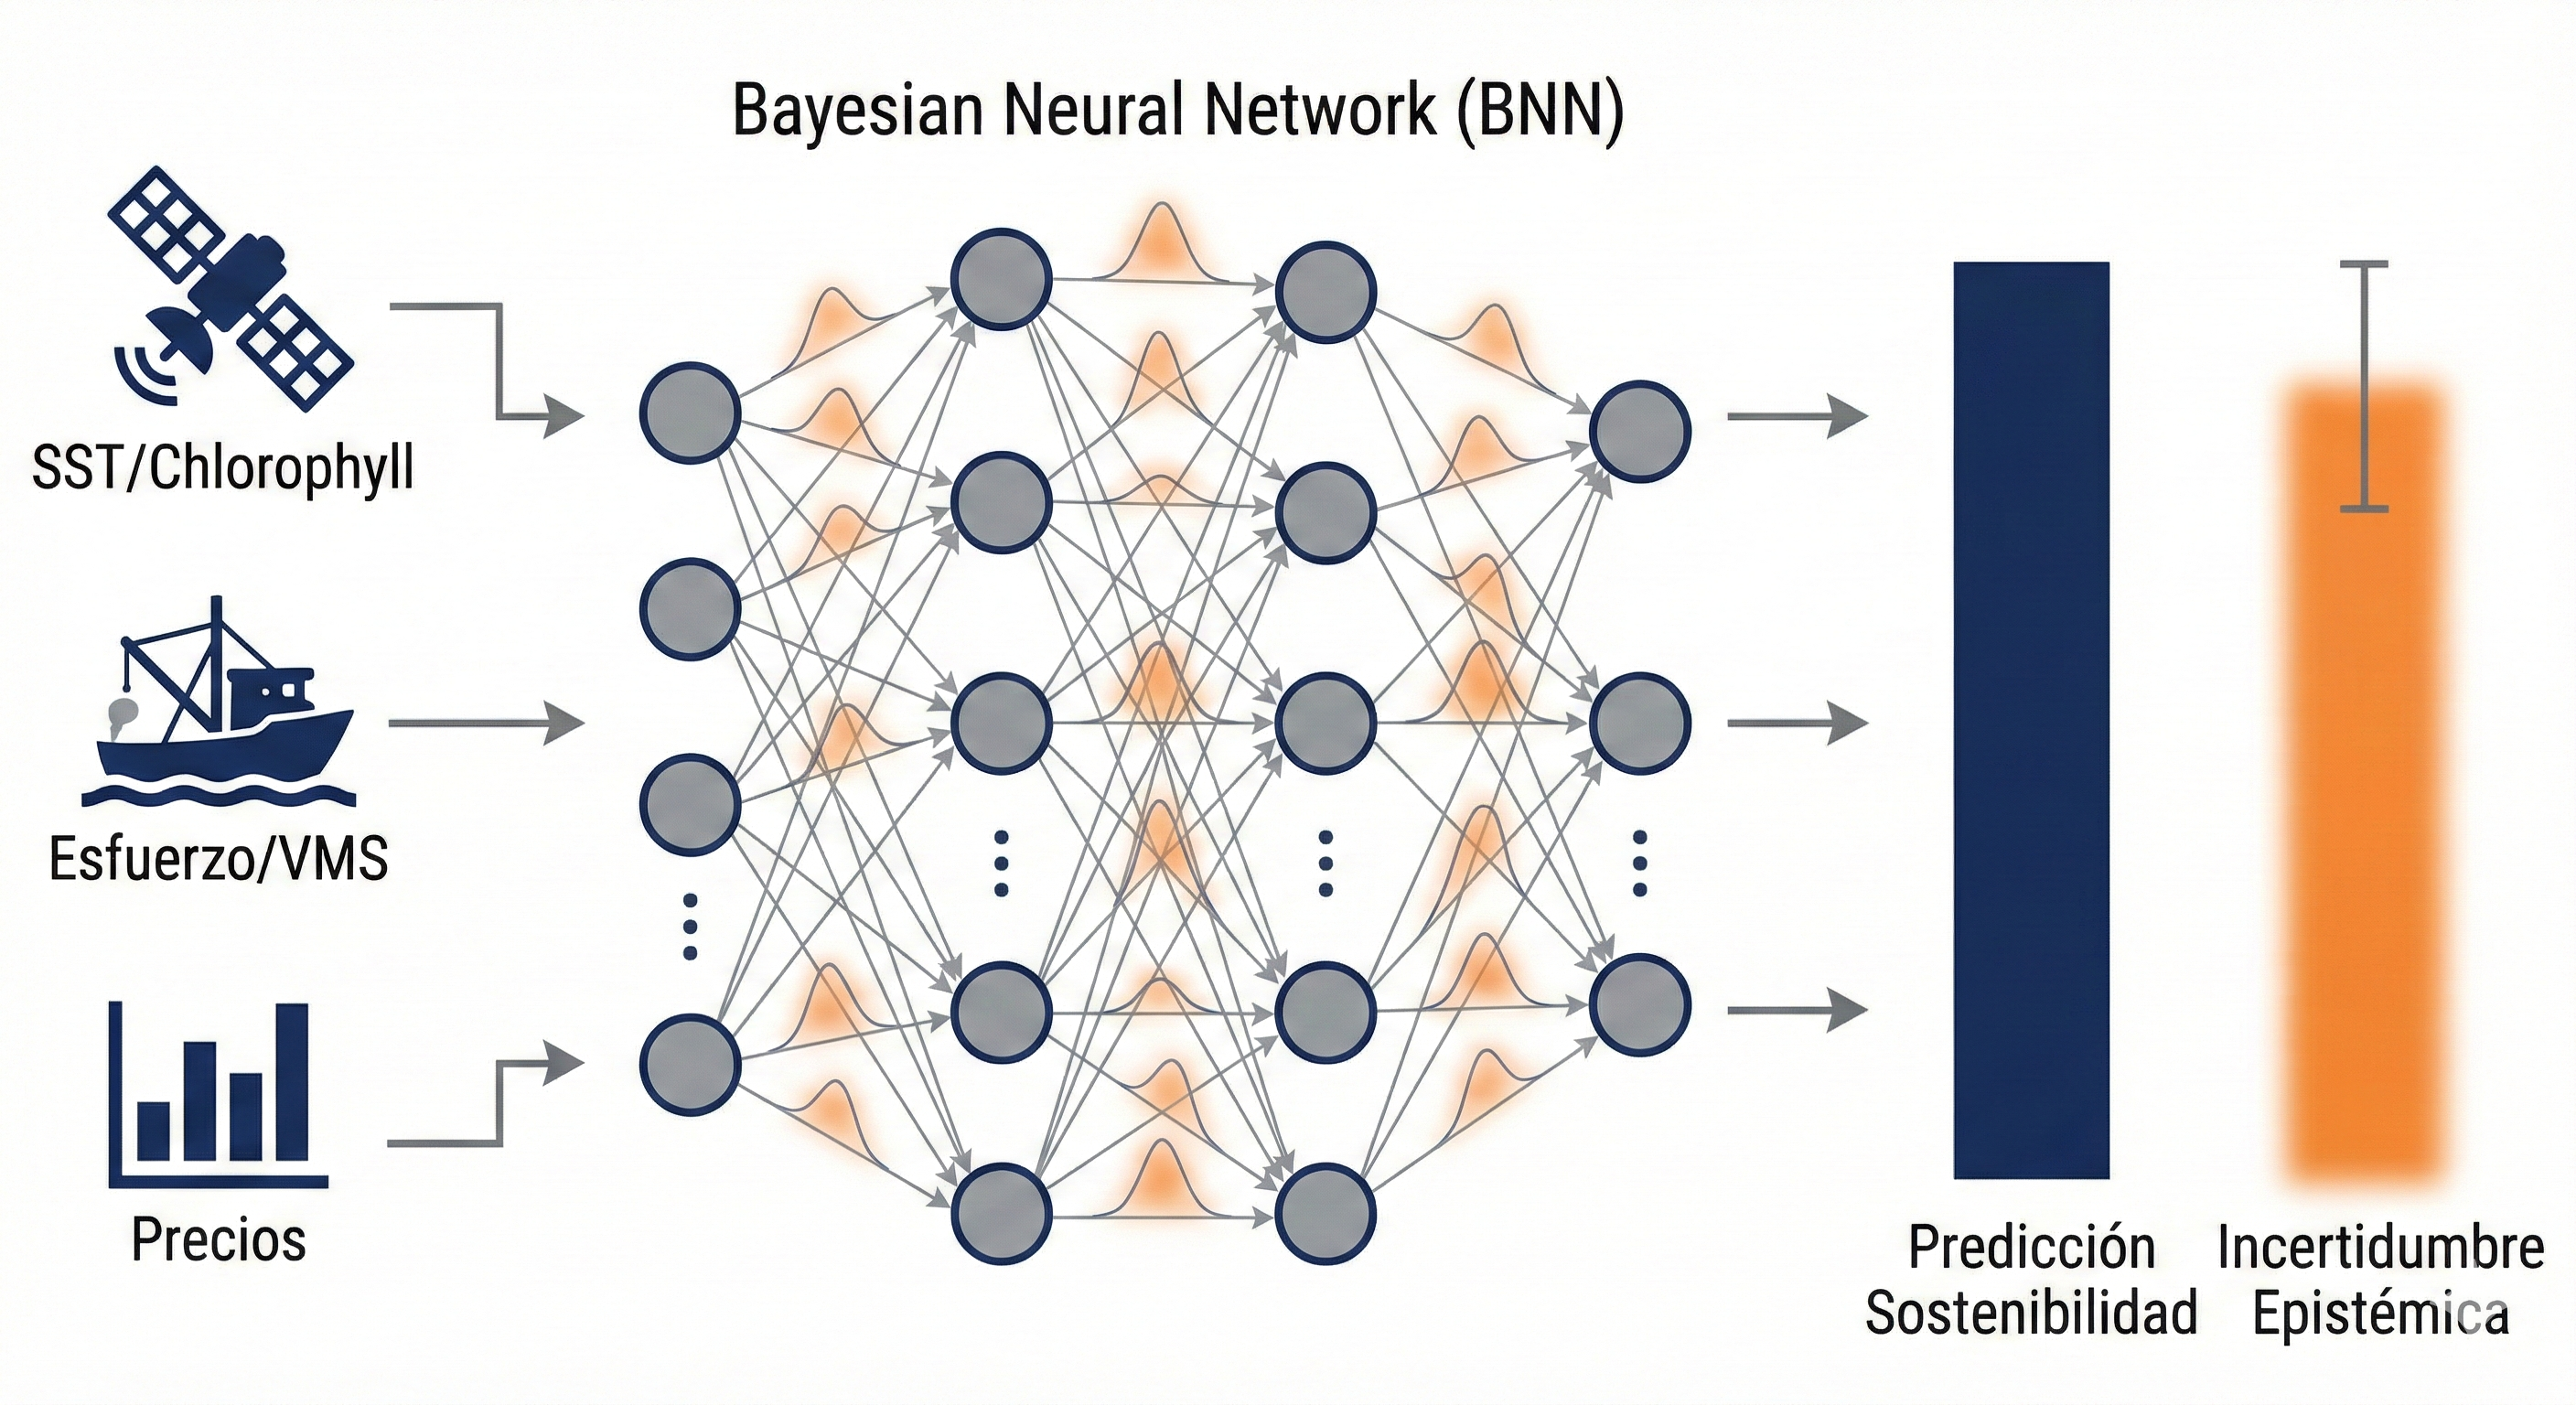
\includegraphics[width=0.85\textwidth]{fig_arquitectura_sistema.png}
\caption{Arquitectura del sistema híbrido neuro-bayesiano propuesto. El flujo integra capas de adquisición de datos (VMS, sensores, satélites), modelado (BNN y redes bayesianas estructurales), inferencia causal (do-calculus), análisis de escenarios y despliegue vía API REST. Las flechas indican el flujo de información entre componentes.}
\label{fig:arquitectura}
\end{figure}

\begin{table}[H]
\centering
\caption{Stack tecnológico del proyecto DL\_Bayesian}
\label{tab:stack}
\begin{tabular}{@{}lll@{}}
\toprule
\textbf{Componente} & \textbf{Tecnología} & \textbf{Función} \\
\midrule
Backend ML & PyTorch + pgmpy & BNN y redes bayesianas \\
API & FastAPI & Endpoints REST \\
MLOps & MLFlow + Optuna & Tracking y optimización \\
Inferencia causal & do-calculus & Análisis de intervenciones \\
Deploy & Docker + AWS ECS & Producción escalable \\
\bottomrule
\end{tabular}
\end{table}

\subsection{Redes Neuronales Bayesianas para predicción con incertidumbre}

El núcleo del Deep Learning Bayesiano implementado asigna distribuciones de probabilidad a cada peso de la red. Para la implementación se utiliza Inferencia Variacional mediante algoritmos como ADVI (Automatic Differentiation Variational Inference), permitiendo escalar modelos bayesianos a conjuntos de datos masivos.

La salida del sistema para cada predicción incluye:

\begin{itemize}[noitemsep]
    \item Clasificación: Sostenible / No Sostenible
    \item Probabilidad asociada
    \item Intervalo de credibilidad (cuantificación de incertidumbre)
\end{itemize}

Esto se alinea directamente con el principio precautorio requerido por la certificación MSC y los puntos de referencia $B_{40\%}$ adoptados para centolla.

\subsection{Análisis causal y simulación de intervenciones}

El módulo de análisis causal implementa do-calculus para responder preguntas contrafactuales críticas para la gestión:

\begin{quote}
\textit{``Si reduzco el esfuerzo pesquero en 20\%, ¿cómo cambia la probabilidad de sostenibilidad?''}
\end{quote}

\begin{figure}[H]
\centering
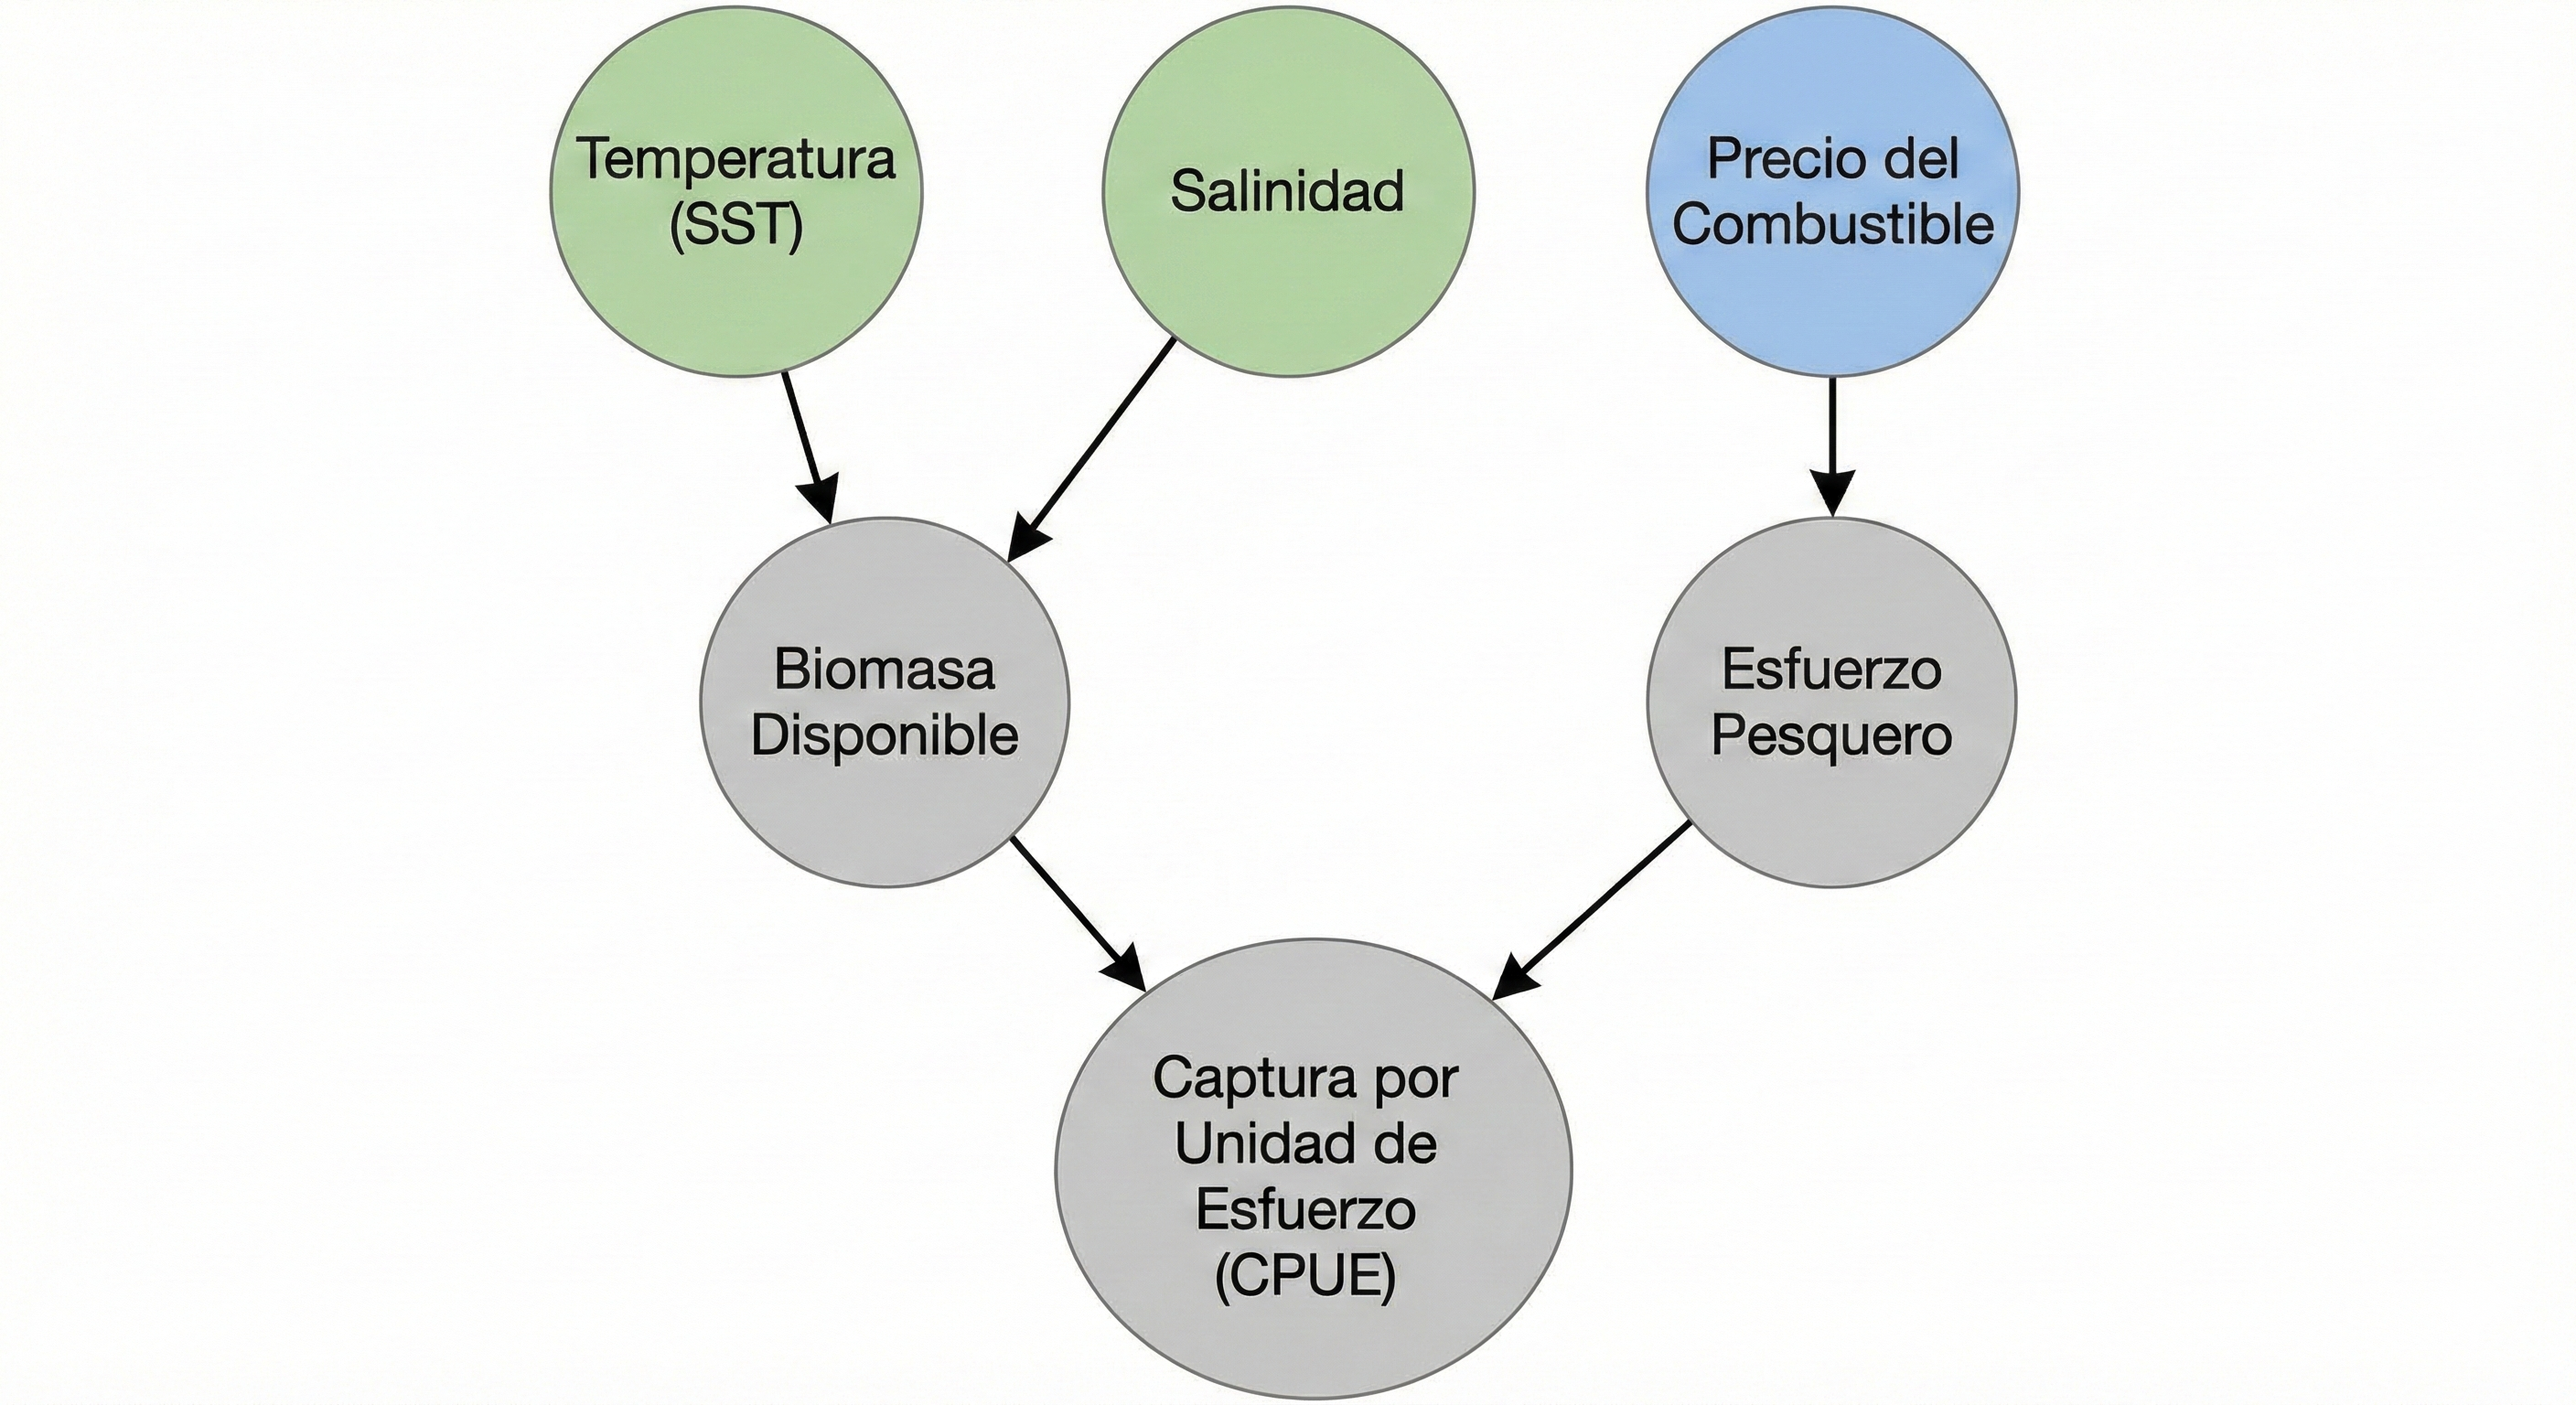
\includegraphics[width=0.80\textwidth]{fig_dag_causal.png}
\caption{Grafo acíclico dirigido (DAG) de la pesquería de centolla implementado en el sistema. Los nodos representan variables ambientales (temperatura, salinidad, clorofila), operativas (esfuerzo pesquero, CPUE, tamaño de flota) y económicas (costos, precios). Las aristas codifican relaciones causales hipotéticas derivadas de conocimiento experto del dominio. La variable objetivo (Sostenibilidad) integra las influencias de todas las capas.}
\label{fig:dag_causal}
\end{figure}

\begin{figure}[H]
\centering
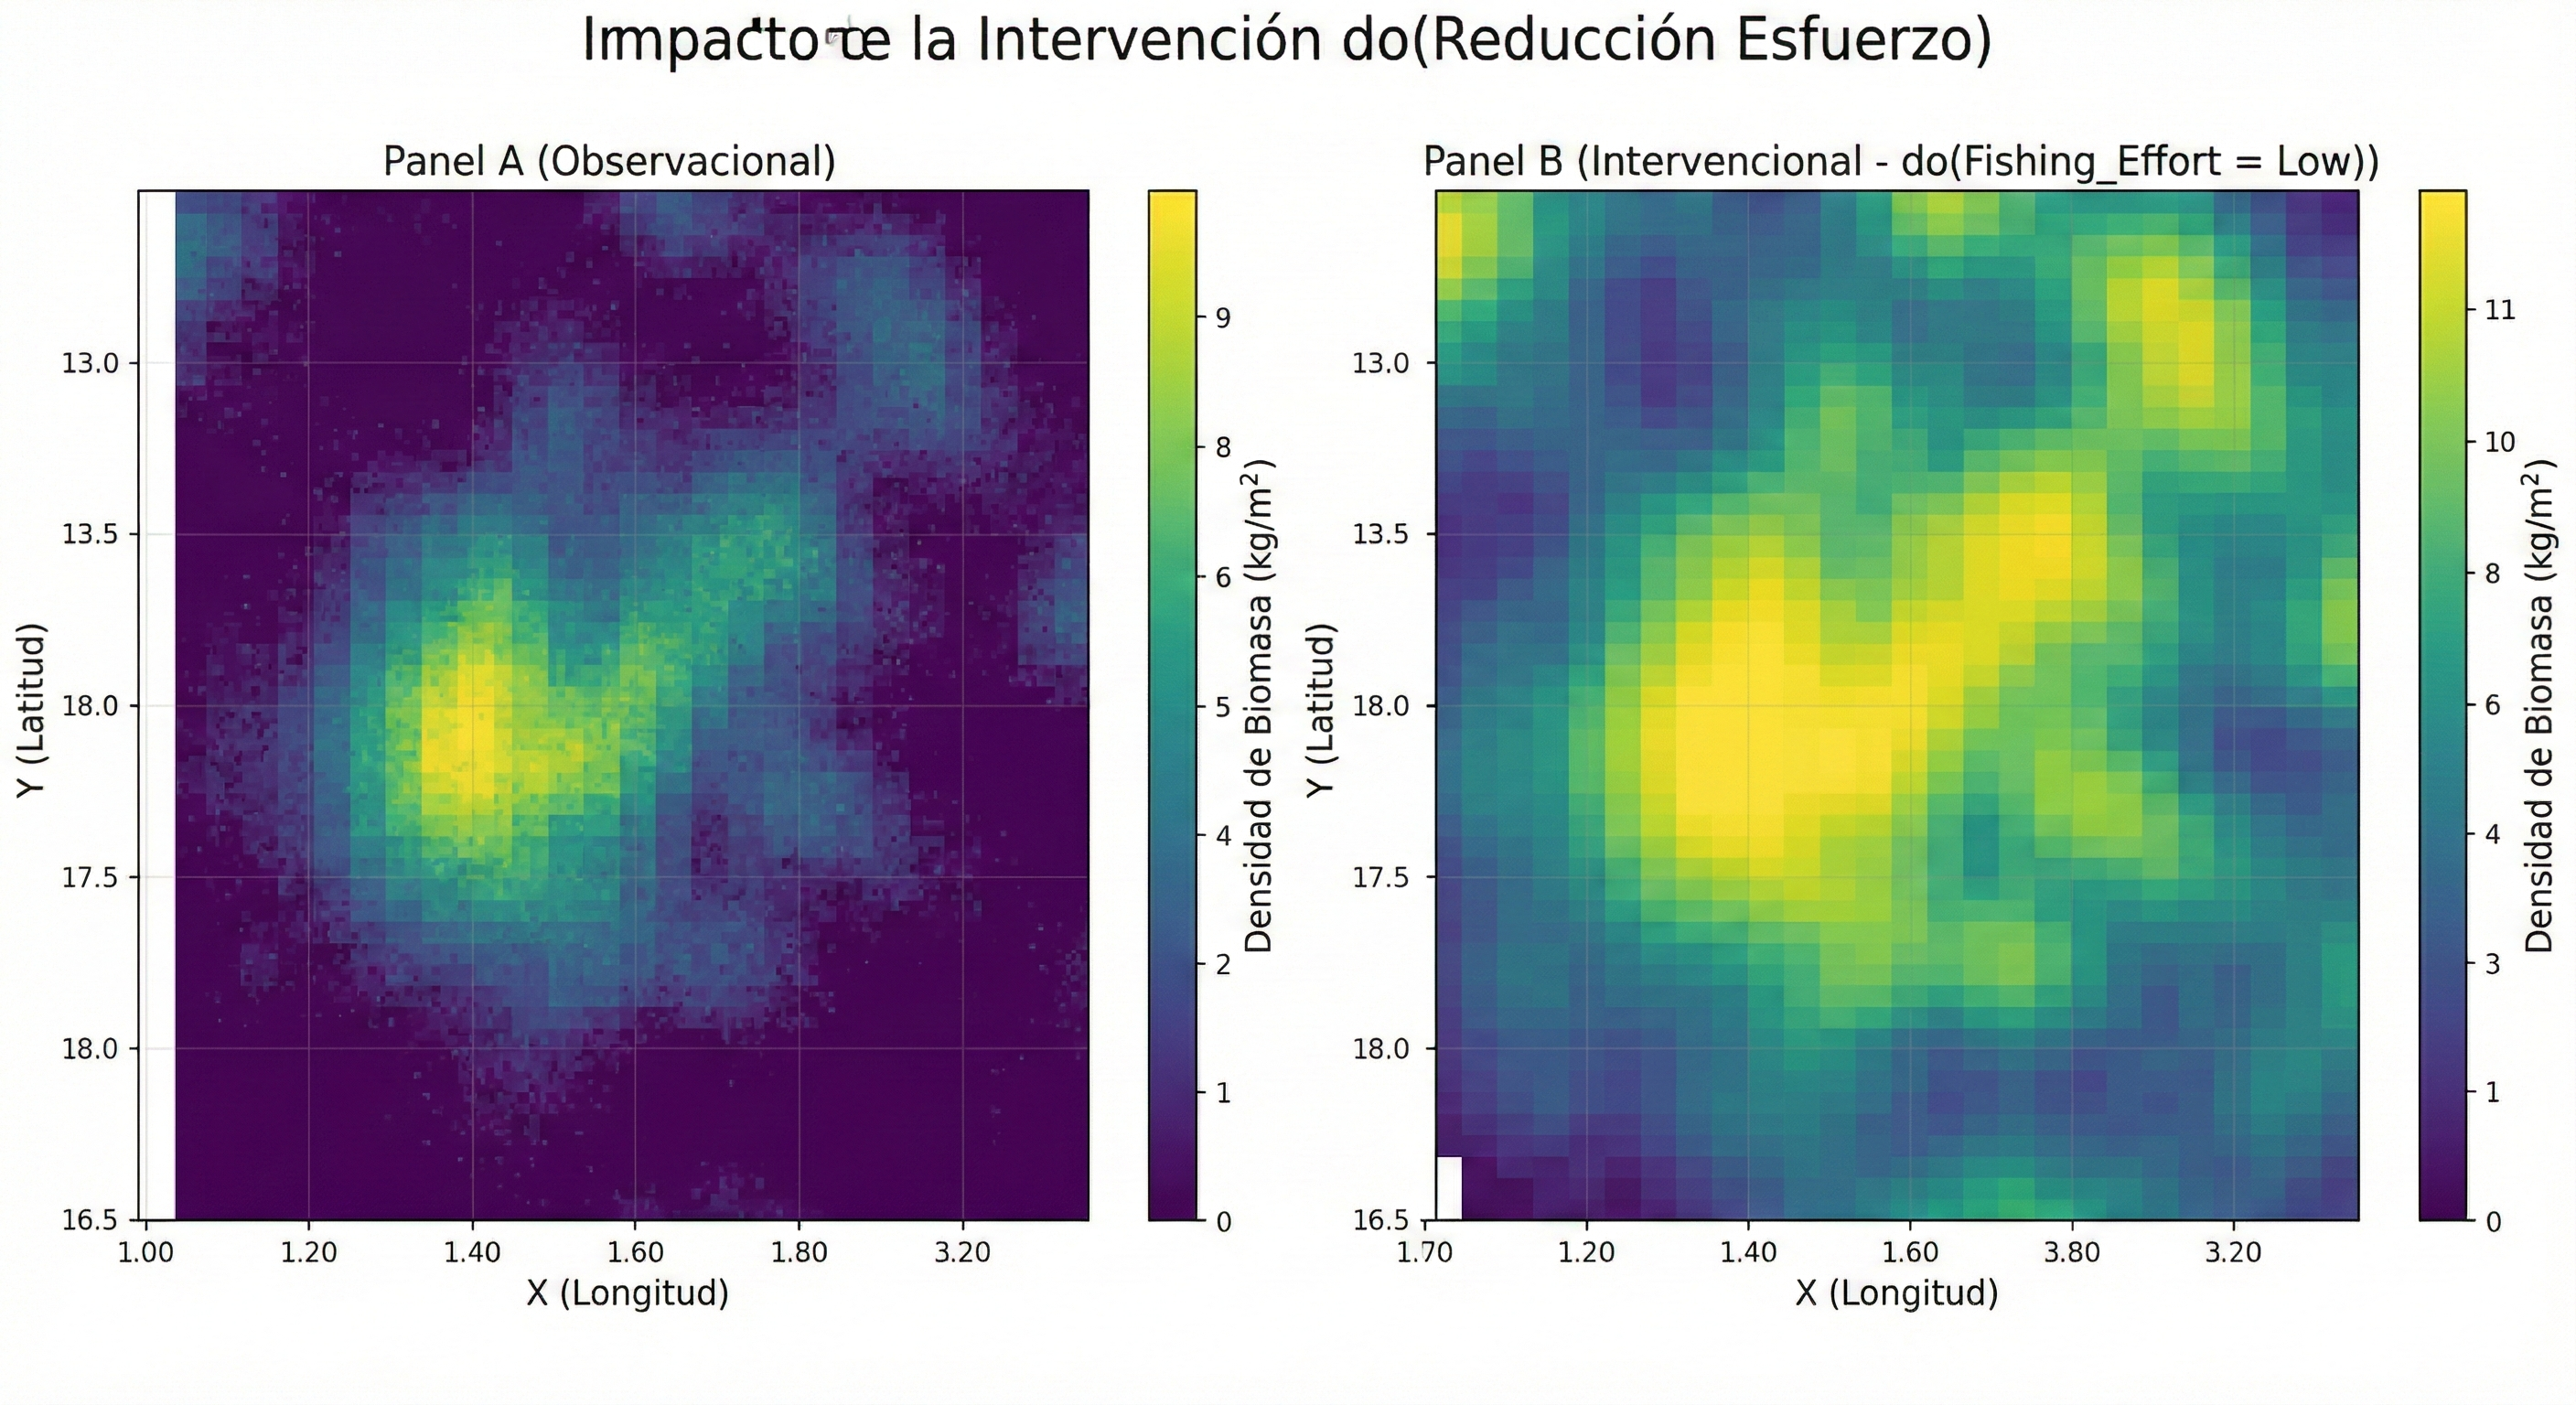
\includegraphics[width=0.80\textwidth]{fig_contrafactuales.png}
\caption{Visualización de escenarios contrafactuales mediante do-calculus. El panel muestra cómo varía la distribución de probabilidad de sostenibilidad bajo diferentes intervenciones simuladas: reducción del esfuerzo pesquero, modificación de la captura total admisible (TAC) y restricciones temporales. Las distribuciones posterior permiten comparar escenarios de manejo antes de su implementación.}
\label{fig:contrafactuales}
\end{figure}

Esta capacidad permite evaluar escenarios de manejo antes de implementarlos, simulando efectos de cambios en TAC, modificaciones a la talla mínima, o restricciones temporales adicionales.

\subsection{Limitaciones y naturaleza de los datos}

Es fundamental explicitar que el proyecto \software{DL\_Bayesian}, en su estado actual, constituye una \textbf{prueba de concepto metodológica basada íntegramente en datos sintéticos} generados algorítmicamente. Las variables ambientales (temperatura superficial del mar, salinidad, clorofila-\textit{a}), operativas (esfuerzo pesquero, CPUE, tamaño de flota) y económicas (costos operativos, precios de mercado, márgenes) fueron simuladas mediante distribuciones estadísticas cuyos rangos y correlaciones se calibraron a partir de valores reportados en la literatura para pesquerías de crustáceos patagónicos \citep{Lovrich1999, Canales2020}.

Las relaciones causales modeladas en el sistema---incluyendo la estructura de los grafos acíclicos dirigidos (DAGs) y las distribuciones de probabilidad condicional---son \textbf{simuladas a partir de conocimiento experto del dominio} y no derivadas empíricamente de observaciones de campo. Si bien esta aproximación permite demostrar la viabilidad técnica de la arquitectura propuesta y validar el flujo completo del sistema (desde la ingesta de datos hasta la inferencia causal y el despliegue vía API), los resultados numéricos específicos no deben interpretarse como estimaciones reales del estado del stock o de la sostenibilidad de la pesquería.

La validación con datos reales de la pesquería de centolla, provenientes de campañas de investigación del INIDEP, registros históricos del CADIC en Canal Beagle, y datos operativos del sistema SIFIPA, constituye el objetivo central de la \textbf{Fase 1 de la agenda de I+D+i propuesta (2026--2027)}. Esta fase requerirá, además, la calibración de los priors bayesianos contra series temporales observadas y la evaluación de la capacidad predictiva del sistema frente a los modelos de evaluación de stock tradicionales actualmente en uso.

% ----------------------------------------------------------------------------
% 5. BRECHA TECNOLÓGICA
% ----------------------------------------------------------------------------

\section{Brecha Tecnológica en Argentina y Oportunidades}

Argentina ha avanzado en digitalización básica de pesquerías mediante el SIFIPA (Sistema Federal de Información de Pesca y Acuicultura, 2020) y el sistema GUARDACOSTAS de Prefectura Naval. Sin embargo, la implementación de inteligencia artificial para evaluación de stocks permanece ausente.

\begin{table}[H]
\centering
\caption{Brecha tecnológica en pesquerías argentinas}
\label{tab:brecha}
\begin{tabular}{@{}lll@{}}
\toprule
\textbf{Tecnología} & \textbf{Argentina} & \textbf{Países líderes} \\
\midrule
Bitácoras electrónicas & Implementado (2019+) & Estándar \\
Monitoreo satelital (VMS) & Operacional & Estándar global \\
Monitoreo electrónico (cámaras) & Solo pilotos & Amplio despliegue \\
IA para evaluación de stocks & \textbf{NO IMPLEMENTADO} & Operacional \\
BNN en pesquerías & \textbf{NO EXISTE} & \textbf{NO EXISTE} \\
\bottomrule
\end{tabular}
\end{table}

La última fila de la Tabla \ref{tab:brecha} destaca la oportunidad más significativa: las Bayesian Neural Networks no han sido aplicadas en pesquerías a nivel global. Esto posiciona al proyecto \software{DL\_Bayesian} como potencial contribución original a la literatura científica.

Las barreras identificadas para implementación incluyen:

\begin{itemize}[noitemsep]
    \item \textbf{Financiamiento}: Altos costos de inversión inaccesibles para PyMEs
    \item \textbf{Fragmentación institucional}: Jurisdicción dividida nacional/provincial
    \item \textbf{Expertise}: Brecha en capacidades de ciencia de datos
    \item \textbf{Conectividad}: Limitaciones para reportes en tiempo real
\end{itemize}

% ----------------------------------------------------------------------------
% 6. PROPUESTA I+D+i
% ----------------------------------------------------------------------------

\section{Propuesta de Línea de I+D+i}

Se propone una agenda de investigación estructurada en tres fases:

\subsection*{Fase 1 (2026-2027): Validación y calibración}
\begin{itemize}[noitemsep]
    \item Adaptación del framework \software{DL\_Bayesian} a datos reales de centolla
    \item Integración con series históricas INIDEP y campañas CADIC
    \item Validación cruzada contra evaluación de stock tradicional
\end{itemize}

\subsection*{Fase 2 (2027-2028): Implementación piloto}
\begin{itemize}[noitemsep]
    \item Despliegue de sistema de clasificación sexo/talla basado en CNN
    \item Integración con sistema de observadores a bordo
    \item Dashboard de soporte a decisiones para gestores provinciales
\end{itemize}

\subsection*{Fase 3 (2028-2029): Escalamiento y transferencia}
\begin{itemize}[noitemsep]
    \item Extensión a otras pesquerías patagónicas (langostino, merluza negra)
    \item Publicación de herramientas como código abierto (GitHub)
    \item Capacitación de recursos humanos en INIDEP y universidades regionales
\end{itemize}

% ----------------------------------------------------------------------------
% 7. CONCLUSIONES
% ----------------------------------------------------------------------------

\section{Conclusiones}

La pesquería de centolla patagónica presenta características únicas que la posicionan como caso piloto ideal para implementación de tecnologías de ciencia de datos en Argentina:

\begin{itemize}[noitemsep]
    \item Flota pequeña y controlable (4-5 buques)
    \item Certificación MSC que requiere mejora continua
    \item Base robusta de conocimiento biológico
    \item Sistema de datos en desarrollo (SIFIPA)
    \item Cobertura de observadores del 85\%
\end{itemize}

Las metodologías revisadas---CNN para clasificación automatizada, LSTM para predicción temporal, BRT para distribución espacial, y modelos bayesianos para evaluación de stocks---están suficientemente maduras para transferencia tecnológica. La ausencia de BNNs en la literatura pesquera representa una oportunidad para contribución científica original que el proyecto \software{DL\_Bayesian} está posicionado para capitalizar.

La implementación requerirá colaboración institucional entre CADIC (expertise biológico), INIDEP (datos pesqueros), universidades con capacidad en ciencia de datos (UTN), y potencialmente socios internacionales como AZTI (España) o programas FAO.

Como expresó Roberto Arlt: \textit{``El futuro es nuestro por prepotencia de trabajo''}. La transformación del sector pesquero argentino mediante inteligencia artificial bayesiana representa un paso fundamental para asegurar que la riqueza del Atlántico Sur sea gestionada con la precisión y prudencia que el siglo XXI demanda.

% ----------------------------------------------------------------------------
% AGRADECIMIENTOS
% ----------------------------------------------------------------------------

\section*{Agradecimientos}

El autor agradece a los colegas del Laboratorio de Crustáceos del CADIC-CONICET por las discusiones que inspiraron este trabajo, y a la comunidad de ciencia de datos pesquera por su compromiso con la innovación abierta.

% ----------------------------------------------------------------------------
% MATERIAL SUPLEMENTARIO
% ----------------------------------------------------------------------------

\section*{Material Suplementario}

El código fuente del proyecto está disponible como repositorio de código abierto:

\begin{center}
\url{https://github.com/arielgiamportone/fisheries-sustainability-mlops}
\end{center}

El repositorio incluye notebooks demostrativos, documentación técnica completa, y datos de ejemplo para reproducibilidad. Adicionalmente, un curso educativo basado en este proyecto está disponible en la comunidad Pesqueros en IA: \url{https://github.com/PesquerosEnIA/curso-dl-bayesiano-pesquerias}.

% ----------------------------------------------------------------------------
% LISTA DE FIGURAS Y TABLAS
% ----------------------------------------------------------------------------

\listoffigures
\listoftables

% ----------------------------------------------------------------------------
% REFERENCIAS
% ----------------------------------------------------------------------------

\bibliographystyle{apalike}

\begin{thebibliography}{99}

\bibitem[Calcagno et al., 2005]{Calcagno2005}
Calcagno, J.A., Lovrich, G.A., Thatje, S., Nettelmann, U., \& Anger, K. (2005).
\newblock Larval and early juvenile development of \textit{Lithodes santolla} (Molina, 1782) (Decapoda: Anomura: Lithodidae) reared at different temperatures in the laboratory.
\newblock \textit{Helgoland Marine Research}, 59, 97--107.

\bibitem[Canales et al., 2020]{Canales2020}
Canales, C., Wyngaard, J., \& Laco, M.L. (2020).
\newblock First quantitative stock assessment for southern king crab in the Central Patagonian Sector.
\newblock \textit{INIDEP Technical Report}.

\bibitem[Chen et al., 2023]{Chen2023}
Chen, H., Liu, Y., Zhang, C., \& Wang, X. (2023).
\newblock Chinese mitten crab detection and gender classification method based on GMNet-YOLOv4.
\newblock \textit{Computers and Electronics in Agriculture}, 215, 108368.

\bibitem[FAO, 2024]{FAO2024}
FAO. (2024).
\newblock \textit{The State of World Fisheries and Aquaculture 2024}.
\newblock Rome: Food and Agriculture Organization of the United Nations.

\bibitem[Kühn et al., 2024]{Kuhn2024}
Kühn, B., Kleisner, K., Osgood, G., \& Watson, R. (2024).
\newblock Machine Learning Applications for Fisheries---At Scales from Genomics to Ecosystems.
\newblock \textit{Reviews in Fisheries Science \& Aquaculture}.

\bibitem[Lovrich \& Vinuesa, 1999]{Lovrich1999}
Lovrich, G.A., \& Vinuesa, J.H. (1999).
\newblock Reproductive potential of the lithodids \textit{Lithodes santolla} and \textit{Paralomis granulosa} (Anomura, Decapoda) in the Beagle Channel, Argentina.
\newblock \textit{Scientia Marina}, 63, 95--105.

\bibitem[Mäntyniemi et al., 2015]{Mantyniemi2015}
Mäntyniemi, S., Uusitalo, L., Peltonen, H., Haapasaari, P., \& Kuikka, S. (2015).
\newblock General state-space population dynamics model for Bayesian stock assessment.
\newblock \textit{ICES Journal of Marine Science}, 72, 2209--2222.

\bibitem[Punt \& Hilborn, 1997]{Punt1997}
Punt, A.E., \& Hilborn, R. (1997).
\newblock Fisheries stock assessment and decision analysis: the Bayesian approach.
\newblock \textit{Reviews in Fish Biology and Fisheries}, 7, 35--63.

\bibitem[Punt et al., 2013]{Punt2013}
Punt, A.E., Huang, T., \& Maunder, M.N. (2013).
\newblock Review of integrated size-structured models for stock assessment of hard-to-age crustacean and mollusc species.
\newblock \textit{ICES Journal of Marine Science}, 70, 16--33.

\bibitem[Trifonova et al., 2017]{Trifonova2017}
Trifonova, N., Kenny, A., Maxwell, D., Duplisea, D., Fernandes, J., \& Tucker, A. (2017).
\newblock Predicting ecosystem responses to changes in fisheries catch, temperature, and primary productivity with a dynamic Bayesian network model.
\newblock \textit{ICES Journal of Marine Science}, 74, 1334--1343.

\bibitem[Wang et al., 2018]{Wang2018}
Wang, G., Chen, Y., An, P., Hong, H., Hu, J., \& Huang, T. (2018).
\newblock Convolutional neural network guided blue crab knuckle detection for autonomous crab meat picking machine.
\newblock \textit{Computers and Electronics in Agriculture}, 153, 267--275.

\bibitem[Winker et al., 2018]{Winker2018}
Winker, H., Carvalho, F., \& Kapur, M. (2018).
\newblock JABBA: Just Another Bayesian Biomass Assessment.
\newblock \textit{Fisheries Research}, 204, 275--288.

\end{thebibliography}

\end{document}
